%
% File acl2016.tex
%
%% Based on the style files for ACL-2015, with some improvements
%%  taken from the NAACL-2016 style
%% Based on the style files for ACL-2014, which were, in turn,
%% Based on the style files for ACL-2013, which were, in turn,
%% Based on the style files for ACL-2012, which were, in turn,
%% based on the style files for ACL-2011, which were, in turn, 
%% based on the style files for ACL-2010, which were, in turn, 
%% based on the style files for ACL-IJCNLP-2009, which were, in turn,
%% based on the style files for EACL-2009 and IJCNLP-2008...

%% Based on the style files for EACL 2006 by 
%%e.agirre@ehu.es or Sergi.Balari@uab.es
%% and that of ACL 08 by Joakim Nivre and Noah Smith

\documentclass[11pt]{article}
\usepackage{acl2016}
\usepackage{times}
\usepackage{url}
\usepackage{latexsym}
\usepackage{amsmath}
\usepackage{amssymb}
\usepackage{color,soul}
\usepackage[pdftex]{graphicx}
\usepackage{todonotes}

%\aclfinalcopy % Uncomment this line for the final submission
%\def\aclpaperid{***} %  Enter the acl Paper ID here

%\setlength\titlebox{5cm}
% You can expand the titlebox if you need extra space
% to show all the authors. Please do not make the titlebox
% smaller than 5cm (the original size); we will check this
% in the camera-ready version and ask you to change it back.

\newcommand\BibTeX{B{\sc ib}\TeX}
\newcommand\toin{\todo[inline]}

\title{Local Named Entity Disambiguation with Neural Attention}

\author{First Author \\
	Affiliation / Address line 1 \\
	Affiliation / Address line 2 \\
	Affiliation / Address line 3 \\
	{\tt email@domain} \\\And
	Second Author \\
	Affiliation / Address line 1 \\
	Affiliation / Address line 2 \\
	Affiliation / Address line 3 \\
	{\tt email@domain} \\}

\date{}

\begin{document}
\maketitle
\begin{abstract}
	Hello, My name is. what? my name is. who?
	My name is. what? my name is. who?
	My name is. what? my name is. who?
	My name is. what? my name is. who?
	My name is. what? my name is. who?
	My name is. what? my name is. who?
	My name is. what? my name is. who?
	My name is. what? my name is. who?
	My name is. what? my name is. who?
	My name is. what? my name is. who?
	My name is. what? my name is. who?
	My name is. what? my name is. who?
	My name is. what? my name is. who?
	My name is. what? my name is. who?
	My name is. what? my name is. who? Lorem ipsum.
\end{abstract}



\section{Introduction}

\toin{General comment about citations -- take whatever bibs you can from the ACL anthology: http://aclweb.org/anthology/

The bibs from Google scholar lack a lot of information.}

Named Entity Disambiguation (NED) is the task of linking mentions of entities in text to a given knowledge base, such as Freebase or Wikipedia. NED is a key component in Entity Linking (EL) systems, focusing on the disambiguation task itself, independently from the tasks Named Entity Recognition (detecting mention bounds) and Candidate Generation (retrieving the set of potential candidate entities). NED has been recognized as an important component in semantic parsing \cite{berant2013semantic}, as well as other NLP tasks.

NED algorithms can broadly be divided into local and global approaches. Local algorithms disambiguate each mention independently using local context (e.g. the sentence in which the mention appeared), whereas global approaches assume some coherence among mentions within a single document, and try to disambiguate all mentions simultaneously. Global algorithms have significantly outperformed the local approach on standard datasets \cite{guo2014entity,pershina2015personalized,globerson2016collective}. However, most of these datasets are based on news corpora and Wikipedia, which are naturally coherent, well-structured, and rich in context. Other domains, such as web page fragments, social media \cite{derczynski2015analysis}, or questions \cite{klang2014named}, lack the sufficient coherence and context for global models to pay off.\todo{Potentially give citations for each domain. YOTAM: not sure how to cite these. Is the QA cite good?}

\toin{Question: could we create a similar dataset of questions or tweets? I think this would provide a much more versatile benchmark, and perhaps allow more cases for your method to shine.}

\toin{Insert example of incoherent context *from the dataset*. This will convince the reader that your problem is real.}

In this work, we investigate the task of NED in a setting where only local and noisy context is available. In particular, we create a dataset of 3.2M short text fragments extracted from web pages, each containing a mention of a named entity. Our dataset contains 18K unique mentions linking to over 100K unique entities. This dataset is significantly larger than previously collected ones such as CoNLL-YAGO \cite{hoffart2011robust}, TAC KBP \cite{ji2010overview} and ACE 2010 \cite{bentivogli2010extending}. 

"She's always been a bit burlesque

allowing us to train a deep neural model for the task.
\todo{Why are you citing Hoffart 2011 if the task is from 2003? YOTAM: They were the ones to annotate it for NED}
\todo{Also, is there a better name for the dataset? CoNLL is the conference's name. I'v seen CoNLL-YAGO}

\toin{Potentially missing from previous paragraph: how do existing models perform on this dataset? Do they fail? You need to convince that there is a real *need* for a new model, and that the neural approach indeed addresses some of the shortcomings of the existing SotA.}

We propose a novel neural network architecture based on Recurrent Neural Networks (RNNs) with an attention mechanism, where the RNN units model textual context as a sequence and the attention mechanism gives importance to contextual signals based on the specific candidate entity being evaluated. Our model differs from non-neural approaches by automatically learning feature representations for entity and context, allowing it to extract features from noisy and unexpected context patterns where it can be hard to manually design useful features. We differ from existing neural-based approaches by accounting for the sequential nature of textual context using RNNs and by devising an attention model that can reduce the impact of noise by assigning weights to different contextual signals based on the specific candidate entity being evaluated.
\toin{Good! This explanation is much more compelling. Relating to the previous comment, do you have some analysis that shows where the previous models fail, and whether your model addresses (even partially) this failure?

For example, are there cases where the disambiguating information is far from the mention, and therefore ignored/forgotten by non-RNN models? How many of these cases exist in your dataset? Does your model significantly improve upon them?}

We also describe a novel method for initializing word and entity embeddings used in our model and demonstrate its importance for model performance and training efficiency. \todo{YOTAM: training taking forever but approaching performance with initialization}

We demonstrate our model greatly outperforms existing state-of-the-art NED algorithms on our web based dataset, showing that existing state-of-the-art methods are not optimal in such settings, and that RNNs with attention can better model noisy and short context. In addition, we evaluate our algorithm on the CoNLL-YAGO dataset \cite{hoffart2011robust}, a dataset of annotated newswire articles, where it yields comparable performance to other state-of-the-art local methods. We conclude that RNNs with attention are well-suited for local disambiguation in clean and well-structured corpora, but that there is still much room for improvement in real world scenarios where text is short, noisy, and less coherent.

\section{Background}

\subsection{Related Work}

\toin{This section is a bit messy... Not sure I understand the flow. What are we trying to communicate here? Also, does it make the paper self-contained? The background should provide a reader who is not familiar with NED (but is from the general NLP/ML community) the necessary background information to be able to understand your contribution.}

The first attempt to use Wikipedia as a knowledge base for local disambiguation was offered by Busco and Pasca back in 2006 \cite{Bunescu2006}. \newcite{hoffart2011robust} suggested a collective global disambiguation graph-based framework, named AIDA, which employed mention, context and coherency models. Similar models were exploited in other global algorithms, such as the GLOW and the Relational Inference systems for the task of Wikification \cite{Ratinov2011,Cheng2013}. \newcite{chisholm2015entity} incorporated web-link data from the Wikilinks dataset \cite{Singh2012} with Wikipedia to train a model for entity linking. Even though demonstrating superior results on well structured evaluations, such as CoNLL, the study does not discuss its performance on the web-link mentions, which presents a very interesting challenge. Also, they choose to model textual context in a Bag-Of-Word (BOW) fashion, eliminating any compositional information of the text. This approach is very different from our suggested recurrent network which allows to capture sematnic information between context words. \todo{I didn't know that someone had already used Wikilinks for NED (although as training). We must state this explicitly, and emphasize the difference/contribution of your work. Noam: Done} More recently, a selective-context model \cite{Lazic2015} has shown that only few context words are informative for the tasks of disambiguation.

In the aforementioned studies two important observations stand out and influenced our algorithmic approach. First, it has been shown that local disambiguation techniques produce a hard baseline to beat even by global NED extensions, which are not even engaged in most disambiguation challenges of traditional NED data sets \cite{Ratinov2011,hoffart2011robust}. This observation, which seems intuitive to the human reader, has led us to concentrate on generating a strong local context-based disambiguation solution. Moreover, following the results of Lazic et al. we designed our model to have an attention mechanism, for reducing the effect of non-informative neighboring text.

Maybe the first attempt of using Deep Neural Networks (DNN) for NED was led by He et al. \cite{He2013}, which learned a similarity measure between mention-context structures and candidates from Wikipedia using stacked autoencoders. Recent studies, have suggested Convolutional Neural Nets (CNN) architectures for learning semantic similarity between all three context, mention and candidate inputs \cite{sun2015modeling,francis2016capturing}. The growing popularity of neural embeddings in NLP related tasks has inspired several researches to jointly map those inputs to the same space using the fantastic word2vec approach \cite{yamada2016joint,Melamud2014}.

\toin{Where is Globerson? Noam: not DNN or ANN}

In this paper, we embed both words and Wikipedia entities in the same space to form input vectors for a Recurrent Neural Network (RNN) model. In this manner, we not only exploit the sequential structure of local surrounding context, but incorporate semantic world knowledge from a much larger corpus in our representation of text. Our novel solution combines these properties with an attention module to produce state-of-the-art local NED results on several datasets.

\subsection{Datasets for NED}

One of the most commonly used evaluation for benchmarking the NED challenge \cite{Globerson2016,Hachey2013,Yamada2016,Pershina2015} is the CoNLL corpus, which was crafted from the CoNLL 2003 Named Entity Recognition (NER) task \shortcite{hoffart2011robust}. CoNLL was composed by manually annotating Reuters newswire articles from 1996. Its contains $1393$ documents from a period of $12$ days split into train, development and test sets. Following previous works we have only evaluated our method on non-NIL mentions.\todo{How was it annotated? By experts? Which KB was it mapped to?}

TAC KBP \cite{ji2010overview} is another popular dataset for testing the performance of disambiguation systems \cite{Chisholm2015,Globerson2016,sun2015modeling}. Similar to CoNLL, it is primarily based on news articles and was specifically designed for the task of entity linking in the Text Analysis Conference (TAC). The most broadly used version for NED is the TAC 2010 data set, which includes a training and test set of $1,070$ and $1,017$ non-NIL mentions, respectively. \footnote{This data set was not available to us, as it is distributed only to TAC participants.}

Some disambiguation systems are also evaluated on the ACE 2005 corpus \cite{Ratinov2011,francis2016capturing}. Being composed out of news reports from various sources, this corpus was extend by connecting and annotating it using Wikipedia \cite{bentivogli2010extending}. It features $16,310$ annotated mentions when only $1,458$ of them have multiple links, hence making them challenging for NED. 

\toin{חבר׳ה, יש פה הרמה להנחתה שאתם לא מנצלים... מה רע בדאטאסטים האלה? מה אתם מחדשים על פניהם?}

\toin{This section provides readers who are less familiar with the literature the necessary information to understand your contribution. Things that need to appear in this section:
	
	- Previous work on NED.
	
	- An in-depth survey of the existing datasets and how they were built.
	
	- Neural work on NED.
	
	At the end of each paragraph/subsection, mention how this work improves upon / differs from what you just discussed.
}

%Deep Neural Networks (DNN) have recently gained traction as state-of-the-art architectures that can model powerful data representations and complex feature interaction. DNNs achieve state-of-the-art results on a wide variety of tasks ranging from image classification \cite{krizhevsky2012imagenet} to machine translation \cite{bahdanau2014neural}. For the task of NED, He at el. \shortcite{he2013learning} used stacked auto-encoders to learn entity and context representations. More recently Sun at el. and Francis-Landau at el. \shortcite{sun2015modeling,francis2016capturing} have proposed models that use convolutional neural networks for modeling and combining representations of a range of input signals and granularities. 

%We propose a novel Deep-Learning based disambiguation algorithm where NED is treated as separating correct entity assignments from corrupt ones given only a local context. Our model is based on Recurrent Neural Networks (RNNs) since they are state-of-the-art language modeling architectures. inspired by Globerson at el \cite{Globerson2016} that showed an attention model is beneficial for NED, we develop a neural attention mechanism to enable the model to decide which contextual signals are most important when considering a specific entity assignment. We as well describe a novel method for initializing word and entity embeddings used in our model and demonstrate its importance.

%To test our method we craft a large-scale dataset of short web fragments containing mentions disambiguated into Wikipedia by thousands of website editors. Our dataset is extracted from a subset of the Wikilinks dataset \cite{singh12:wiki-links} which is re-purposed for NED. It represents a large-scale and difficult task with \hl{count} unique mentions disambiguated into $100K$ unique entities and where context is limited and noisy. We demonstrate our model greatly outperforms existing state-of-the-art NED algorithms on this dataset and in addition examine our algorithm on CoNLL \cite{hoffart2011robust}, a standard NED dataset, and show results comparable to other state-out-the-art methods on a smaller and cleaner dataset.


\section{WiikilinksNED Dataset: Entity Mentions in the Web}
\label{sec:w}

\toin{Think of a cool acronym for this dataset, e.g. WNED - web NED.}

We introduce a new large-scale NED dataset based on text fragments from the web. Our dataset is derived from the Wikilinks corpus \cite{singh12:wiki-links}, which was constructed by crawling the web and collecting hyperlinks (mentions) linking to Wikipedia concepts (entities) and their surrounding text (context). Wikilinks contains 40 million mentions covering 3 million entities, collected from over 10 million web pages. 

Wikilinks can be seen as a large-scale, naturally-occurring, crowd-sourced dataset where thousands of human annotators provide ground truths for mentions of interest. This means that the dataset also contains various kinds of noise, including erroneous ground-truth labels, malformed mentions, and incoherent contexts. The contextual noise in particular presents an interesting test-case that supplements existing datasets such as CoNLL-YAGO \cite{hoffart2011robust}, TAC KBP \cite{ji2010overview} and ACE 2010 \cite{bentivogli2010extending}, since these datasets are all sourced from mostly coherent and well-formed text (news and Wikipedia). Wikilinks therefore emphasizes the need to understand the local context, and marginalizes the utility of coherency-based global approaches. 

To get a sense of textual noise and entity-context coherence we have set up a small experiment where we measured the similarity between entities mentioned in WikilinksNED and their surrounding context. We compared the results to CoNLL-YAGO. We used state-of-the-art word and entity embeddings obtained from Yamada at el \cite{yamada2016joint} and computed cosine similarity between an entity embedding and the mean of context words embeddings. We compared results from all mentions in CoNLL-YAGO to a sample of 10000 web fragments taken from WikilinksNED, using a window of words of size 40 around entity mentions. On CoNLL-YAGO we found the mean similarity to be 0.188 while on WikilinksNED we got 0.163. We believe this result indicates that web fragments in WikilinksNED are indeed less coherent and noisier compared to CoNLL-YAGO documents.

\todo{I agree with the reasoning, but we should have some sort of experiment/analysis to back this claim. YOTAM: what about this?}

We prepared our dataset from the local-context version of Wikilinks,\footnote{\url{http://www.iesl.cs.umass.edu/data/wiki-links}} and resolved ground-truth links from the 7/4/2016\todo{American or international dating? YOTAM: International... How can we make this clear?} dump of Wikipedia \footnote{\url{https://dumps.wikimedia.org/}}. We used the \emph{page} and \emph{redirect} tables for resolution, and kept the database \emph{pageid} column as a unique identifier for Wikipedia entities. We discarded mentions where the ground-truth could not be resolved (only 3\% of mentions).

We collected all pairs of mention $m$ and entity $e$ appearing in the dataset, and computed the number of times $m$ refers to $e$ ($\#(m,e)$), as well as the conditional probability of $e$ given $m$: $P(e|m)=\#(m,e)/\sum_{e'}\#(m,e')$. Examining these distributions revealed many mentions belong to two extremes -- either they had very little ambiguity, or they appeared in the dataset only a handful of times and referred to a different entities 1-2 times each.\todo{Not sure I understand the second case. Example? YOTAM: tried to improve explanation. } We deemed the former to be less interesting for the purpose of NED, and suspected the latter to be noise with high probability. To filter these cases, we kept only mentions for which at least two different entities have 10 mentions each ($\#(m,e) \ge 10$) and consist of at least 10\% of occurrences $P(e|m) \ge 0.1$. This procedure aggressively filtered our dataset and we were left with $3.2M$ mentions.

Finally, we randomly split the data into train (90\%), validation (10\%), and test (10\%), according to domains in order to minimize lexical memorization (see \cite{levy2015supervised}).

\section{Algorithm}

Our DNN model is a discriminative model which takes a pair of local context and candidate entity, and outputs a likelihood for the candidate entity being correct. Both words and entities are represented using embedding dictionaries and we interpret local context as a window-of-words to the left and right of a mention. The left and right contexts are fed into a duo of Attentional RNNs (ARRN) components which process each side and produce a fixed length vector representation. The left context is fed in a forward manner while the right context is fed backwards into the model. Each Attentional RNN uses the candidate entity input to control its attention, allowing it to attend to the most discriminating parts of the context given the candidate at hand. 

The output vectors generated by both Attentional RNNs and the embedding of the entity itself are then fed into a classifier network consisting of a hidden layer and an output layer with two output units and a softmax activation. The output units are trained to emit the likelihood of the candidate being a correct or corrupt assignment by optimizing a cross-entropy loss function. 

We assume our model is only given examples of correct entity assignments during training and therefore automatically generate examples of corrupt assignments. For each $(context,entity)$ pair where $entity$ is a correct assignment for a given $contex$ we produce $k$ corrupt examples with the same $context$ and a corrupt entity uniformly sampled from all entities in the dataset. Using the combined dataset of correct and corrupt examples our algorithm learns to separate correct assignments from the generated corrupt ones.

In our implementation we have set the hidden layer size to be 300 and used a ReLU non-linearity for this layer. Preliminary evaluations showed the width and depth of the classifier to be of little impact on performance, but using a ReLU non-linearity was found to be important. We have also applied dropout with $p=0.5$ to the hidden layer.

\subsection{Attentional RNN component}

\begin{figure}
	\centering 
	\caption{Attentional RNN Architecture}
	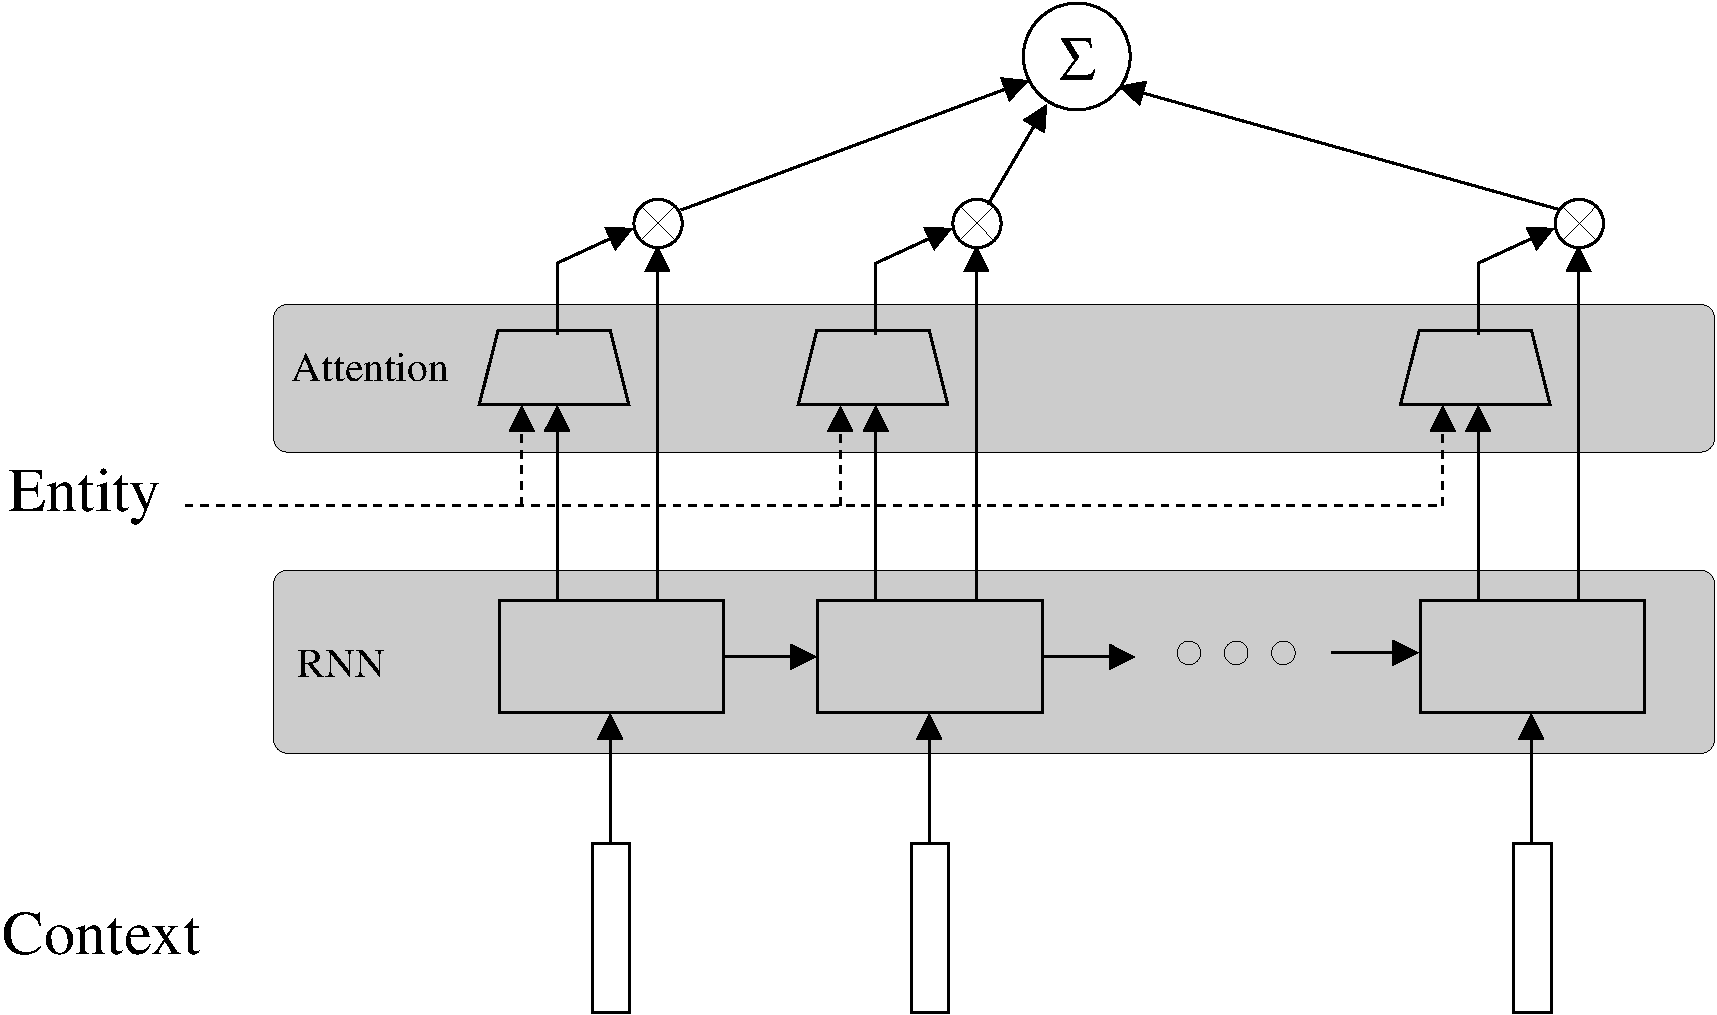
\includegraphics[scale=0.25]{diagrams/RNN_ATTN.pdf}
	\label{fig:arnn}
\end{figure}	

Our Attentional RNN component is based on a general RNN unit fitted with an attention mechanism. The mechanics of the Attentional RNN component are depicted in Figure \ref{fig:arnn}. 
	
Equation \ref{eq1} represents the general semantics of an RNN unit. An RNN reads a sequence of vectors $\{v_t\}$ and maintains a hidden state vector $\{h_t\}$. At each step a new hidden state is computed based on the previous hidden state and the next input vector by a function $f$ parametrized by $\Theta_1$. The output at each step is computed from the hidden state using a function $g$ parametrized by $\Theta_2$. This allows the RNN to 'remember' important signals while scanning the context and to recognize signals spanning multiple words.

\begin{equation}
\label{eq1}
\begin{aligned}
& h_t=f_{\Theta_1}(h_{t-1}, v_t) \\
& o_t=g_{\Theta_2}(h_t)
\end{aligned}
\end{equation}

In out implementation we have used a standard GRU unit \cite{cho2014learning}, however any RNN can be a drop-in replacement. While an RNN unit can be used as-is in our model by feeding the last output vector $o_t$ directly into the classifier network, we have implemented an attention mechanism that allows the model to be aware of the candidate entity it is evaluating when computing an output. Equation \ref{eq2} details the equations governing the attention model.

\begin{equation}
\label{eq2}
\begin{aligned}
& a_t \in \mathbb{R}; a_t=r_{\Theta_3}(o_t, v_{candidate}) \\
& a'_t  = \frac{1}{\sum_{i=1}^{t} \exp\{a_i\}} \exp \{a_t\} \\
& o_{attn}=\sum_{i=1}^{t} a'_t o_t
\end{aligned}
\end{equation}

The main component in equation \ref{eq2} is the function $r$, parametrized by $\Theta_3$, which computes an attention value at each step using $v_{candidate}$, the candidate entity embedding, as a control signal. We use the softmax function to normalize the attention values such that $\sum_{i=1}^{t} a'_i = 1$ and compute the final output $o_{attn}$ as a weighted sum of all the output vectors of the RNN. This allows the attention mechanism to decide on the importance of different context parts when examining a specific candidate. We parametrize our attention function $r$ as a single layer NN as shown in equation \ref{eq3} where $A, B$ are the layer weights and $b$ is a bias term.

\begin{equation}
\label{eq3}
r_{\Theta_3}(o_t, v_{candidate}) = Ao_t + Bv_{candidate} + b \\
\end{equation}


\subsection{Training initial word and entity embeddings}

Training our model implicitly trains its dictionaries of both word and entity embedding by error back-propagation. However, as will be shown in section \ref{experiments}, we have found using pre-trained embeddings to \hl{significantly improve model performance/greatly reduce training time(??)}. To this end we have devised a Skip Gram with Negative Sampling (SGNS) \cite{mikolov2013distributed} based training procedure that simultaneously trains both word and entity vectors in the same embedded space.

We use the word2vecf library\footnote{Available at https://bitbucket.org/yoavgo/word2vecf} by Levy and Goldberg \shortcite{levy2014dependency} that is adapted from word2vec code and allows to train on a dataset made of $(word,context)$ pairs rather then a textual corpus in string format, as is done in the original word2vec. We exploit this to redefine $context$ as a context entity rather then a contextual word. 

We do this by considering each page in Wikipedia to represent a unique entity, enumerated by the $pageid$ identifier in Wikipedia database and having a textual description (the page itself). For each word $\{word_i\}$ in the page we add the pair $(word_i,pageid)$ to our dataset. We however limit our vocabularies by ignoring both rare words that appear less then $20$ times and entities that have less then $20$ words in their description.
	
As shown by Levy and Goldberg \shortcite{levy2014neural} training embeddings on this dataset using SGNS produces word and entity embedding that implicitly factorize the word-entity co-occurrence PPMI matrix. This matrix is closely related to the TFIDF word-entity matrix used by Gabrilovich and Markovitch \shortcite{gabrilovich2007computing} in Explicit Semantic Analysis and found to be useful in a wide array of NLP tasks. 

For our experiments we trained embeddings of length 300 for 10 iterations over the dataset. We used default values for all other parameters in word2vec.

\hl{-needs developing-}

\hl{-show results of the analogies experiment we did indicating semantic structure for the WORD vectors-}

\section{Evaluation} \label{experiments}

In this section we describe the setup used when evaluating our model and present evaluation results for two datasets. We evaluate the effect of initializing word and entity embeddings on our model as well.

In all experiments we trained our model with fixed size left and right contexts, using a 20 word window to each side of the mention. In cases were the context was shorter than the fixed size, we padded it with a special $PAD$ symbol. Further, we filtered stop words according to NLTK's stop-word list.

Model optimization was carried out using standard back propagation and an AdaGrad optimizer \cite{duchi2011adaptive}. We allowed the error to propagate through all parts of the network and fine tune all trainable parameters, including the word and entity embeddings themselves.

\subsection{Wikilinks}

When evaluating a NED system it is required to use some method for generating candidate entities. We use a simple method where given mention $m$ we consider all candidates for whom $P(e|m)>0$, where $P(e|m)$ is the probability of seeing entity $e$ as a ground-truth for mention $m$ in the training corpus. This simple method gives $97\%$ ground-truth recall on the test set. 
We trained for a single \todo{YOTAM: I have better a training regime} epoch with $2.6M$ mentions and $k=5$ for corrupt example generation. Training the model took half a day using a 20-core CPU machine.

We have used the following methods as base line on the Wikilink dataset:

\begin{itemize} 
	\item  \textbf{Yamada et al.} \shortcite{Yamada2016} have created a state-of-the-art NED system that models entity-context similarity with word and entity embedding trained using the skip-gram model. We have obtained trained embeddings from the authors and used statistical features collected from the Wikilinks training set. We used only the local features described by Yamada at el. and trained their ranking model on Wikilinks training set.
	
	\item \textbf{Cheng et al.} \shortcite{Cheng2013} have made publicly available \footnote{Available at https://cogcomp.cs.illinois.edu/page/software\_view/Wikifier } a global method which uses the GLOW system by Ratinov et al. \shortcite{Ratinov2011} for local disambiguation. We compare our results to the ranking step of the algorithm, without the their global component.
	
	\item We include Most Probable Sense (MPS) as a baseline. This baseline picks the entity with the highest $P(e|m)$ as the correct mention. This simple baseline is notoriously known to give competitive results in many NED datasets 
\end{itemize}

Due to long running time of Cheng et al. we have evaluated their method on Wikilink-Small, a smaller version of our test data with $10000$ randomly sampled mentions.

\subsection{CoNLL-YAGO}

CoNLL-YAGO has a training set with $18505$ non-NIL mentions, which preliminary experiments showed is not sufficient to train our model on. We therefore resorted to a more complex training method where we first trained our model on a large corpus of mentions derived from Wikipedia cross-references and then fine tuned the resulting model on CoNLL-YAGO training set. To derive the Wikipedia training corpus we have extracted all cross-reference links from Wikipedia along with their context, resulting in over $80$ million training examples. Due to constrained resources we set $k=1$ for corrupt example generation and trained $1$ epoch, which took around $4$ days to train. The resulting model was then fine-tuned on CoNLL-YAGO training set, where corrupt examples were produced by considering all possible candidates for each mention.
For candidate generation we used the publicly available candidate dataset by Pershina at el. \shortcite{Pershina2015} with over $99\%$ gold sense recall.

We have also found that using traditional statistical and string based features along with our model further improves its performance. We therefor used a setting similar to Yamada et al. \shortcite{yamada2016joint} where a Gradient Boosted Regression Tree was fitted with our models prediction score as a feature along with $7$ other statistical and string based features. The statistical features are prior probability $P(e)$ and conditional probability $P(e|m)$ as described above, along with a feature counting the number of candidates generated for the mention and a feature giving the maximum conditional probability of the entity for all mentions in the document. For string similarity features we used the edit distance between the mention and the entity title in Wikipedia, a feature indicating weather the mention is a prefix or postfix of the entity Wikipedia title and a feature indicating weather the Wikipedia entity title is a prefix or postfix of the mention. Following Yamada we used sklearn's GradientBoostingClassifier implementation \cite{pedregosa2011scikit} with a deviance loss and set the learning rate, number of estimator and maximum depth of a tree to $0.02$, $10000$ and $4$, respectively. 

As a baseline we took the standard Most Probable Sense (MPS) prediction, which corresponds to the $\arg\max_{e\in{{E}}}{P(e|m)}$, where $E$ is the group of all candidate entities.
We also compare to the following papers - Francis-Landau et al. \shortcite{francis2016capturing}, He et al. \shortcite{He2013}, Hoffart et al. \shortcite{hoffart2011robust} and Chisholm et al. \shortcite{Chisholm2015} ,as they are all strong local approaches and a good source for comparison.

\subsection{Results}

Our main evaluation results on the Wikilinks dataset are reported in Table \ref{tab:wikilink}. Our algorithm significantly outperforms both Yamada at el and the base line on this data by substantial margins. This result indicates that the skip-gram model used by Yamada at el. which averages the embedding vectors of all context words is non-optimal compared to our more sophisticated context modeling on this dataset. Our method outperforms the Baseline as well by a very large margin indicating our RNN model is indeed able to capture meaningful contextual features despite the noisy and short context.

\begin{table}[h]
	\begin{center}
		\begin{tabular}{|c| p{1.5cm}|}
			\hline \multicolumn{2}{|c|}{Wikilinks Evaluation} \\
			\hline \bf Model & \bf P@1  \\ \hline
			ARNN  &                              $64.8$ \\
			\bf GBRT: Base + ARNN features & \bf $66.8$ \\
			Yamada at el. &                      $59.8$ \\
			Baseline (MPS) &                     $55.9$ \\
			\hline
		\end{tabular}
	\end{center}
	\caption{\label{tab:wikilink} Evaluation on Web-Fragment data (Wikilinks)}
\end{table}

Table \ref{tab:wikilinks-small} shows evaluation results for the Wikilinks-Small test set. We used a pre-trained model supplied by Cheng at el which, similarly to the setting used for evaluating the GLOW algorithm by Ratinov at el \cite{ratinov2011glow}, was not directly trained on our training set. We believe this explains their poor performance, as Wikilinks is substantially different from other NED datasets both for being noisy and for being annotated by web content authors rather then expert annotators. This last difference results in substantially different annotation patterns.

\begin{table}[h]
	\begin{center}
		\begin{tabular}{|c| p{1.5cm}|}
			\hline \multicolumn{2}{|c|}{Wikilinks-Small Evaluation} \\
			\hline \bf Model & \bf Micro     accuracy  \\ \hline
			\bf ARNN  &  \bf $?$ \\
			Cheng et al. & $~52$ \\
			\hline
		\end{tabular}
	\end{center}
	\caption{\label{tab:wikilinks-small} Evaluation on Web-Fragment data (Wikilinks)}
\end{table}

The micro and macro P@1 scores on CoNLL-YAGO test-b are displayed in table \ref{tab:a}. On this dataset our model achieves reasonable results, however it cannot beat state-of-the-art results since it requires large quantities of training data to properly train the large number of parameters in the model. 

\begin{table}[h]
	\begin{center}
		\begin{tabular}{|p{3.5cm}| p{1.5cm} p{1.5cm}|}
			\hline \multicolumn{3}{|c|}{CoNLL-YAGO test-b (Local methods)} \\
			\hline Model & Micro P@1 & Macro P@1 \\ 
			\hline \multicolumn{3}{|c|}{PPRforNED} \\
			\hline RNN Attention    & $87.3$  & $88.6$ \\
			Yamada et al. local     & $90.9$  & $92.4$ \\
			Baseline (MPS)          & $77$    & $77$ \\
			\hline \multicolumn{3}{|c|}{Yago} \\
			\hline RNN Attention    & $?$  & $?$ \\
			Yamada et al. local     & $87.2$  & $89.6$ \\
			Francis-Landau et al.   & $85.5$  & - \\
			Chisholm et al. local   & $86.1$  & - \\
			\hline Lazic et al.     & $86.4$  & - \\
			\hline
		\end{tabular}
	\end{center}
	\caption{\label{tab:conll} Evaluation on CoNLL-YAGO. Bold font denotes the models offered in this study}
\end{table}


add insights regarding the results and comparison 
\subsection{Model sensitivity}

\toin{Where is ARNN w/o init but with attention?}

\begin{table}[h]
	\begin{center}
		\begin{tabular}{|c| p{1.5cm}|}
			\hline \multicolumn{2}{|c|}{Wikilinks test set} \\
			\hline \bf Model & \bf Micro     accuracy  \\ \hline
			ARNN w/o ESA init. & $61$ \\
			ARNN w/ ESA init. w/o Attention & $64.1$ \\
			ARNN w/ ESA \& Attention & $64.8$ \\ 
			\hline
		\end{tabular}
	\end{center}
	\caption{\label{tab:c} ARNN Model sensetivity}
\end{table}

\section{Conclusions}

\bibliographystyle{acl2016}
\bibliography{_our_submission,_noam_bib}

\end{document}
